\section{Implementation details} \label{sec:implementation}

% The \textsc{Code Contracts} static verifier is invoked by Visual Studio after each compilation. In order to do the instrumentation and let verifier analyze the transformed contracts we need to do it before it reaches the static verifier. This is done modifying the \textsc{Code Contracts} configuration replacing the static verifier with a modified version that does the required instrumentation and then invokes the original verifier.
% 
% \begin{figure}[ht!]
% \begin{center}
% 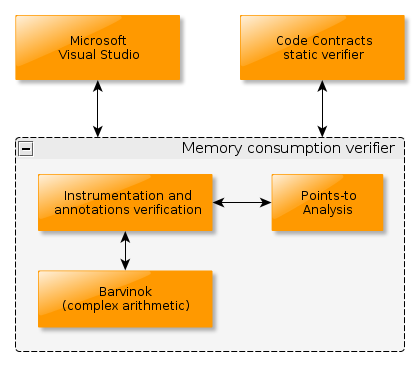
\includegraphics[scale=0.5]{arq.png}
% \end{center}
% %\vspace*{-2em}
% \caption{General architecture of the tool}
% %\vspace*{-1em}
% \label{arq}
% \end{figure}
% 
% Figure \ref{arq} shows the general architecture of the tool. The component labeled \textit{Memory consumption verifier} has the same interface as the \textsc{Code Contracts} verifier, so it can replace it when Visual Studio invokes it. Internally, the \textit{Memory consumption verifier} uses the described algorithms and tools to do the instrumentation and verification, then it invokes the \textsc{Code Contracts} verifier and returns to Visual Studio the verification results.

We developed a Visual Studio extension\footnote{\small Available at: \url{http://lafhis.dc.uba.ar/resourcecontracts}.} that lets developers write memory consumption contracts as  they do with \textsc{Code Contracts} and verify them using its static verifier or run-time checker.
The only prerequisite for the plug-in is having \textsc{Code Contracts} installed, all the other tools used by the memory contracts checker are packaged in the plugin.
We use the Common Compiler Infrastructure (CCI)~\cite{CCI} for code analysis and instrumentation.
%Memory contracts checking can be activated or deactivated in a per-project basis. 
%Once enabled, the memory contracts annotations become available in the project, having autocompletion and inline documentation, just like \textsc{Code Contracts} annotations.

The \textsc{Code Contracts} static checker is invoked by Visual Studio after each compilation. 
In order to transform the code before checking it, we use a wrapper that performs the required instrumentation and then invokes the actual checker. When the plug-in is installed it modifies the \textsc{Code Contracts} configuration in order to setup this wrapper. So far, we have not found a better way to ensure that our tool is invoked before the \textsc{Code Contracts} checker.

